In this chapter, we analyze the fourth experiment group, that is, the impact of having different amounts of clients, per scoring algorithm, in a Blockchain-based Federated Learning (BFS) system. In this set of experiments, all properties of the system are static, except for the amount of clients, which varies between 5, 10, 25 and 50, per each scoring algorithm.

\section{Execution Time, Transaction Cost and Latency}

The first aspects we analyze are the execution times and the transaction costs and latency. These can be visualized in \autoref{fig:clients_metrics}.

Regarding execution times, all scoring algorithms present different growths with the increase of clients. One one hand, no scoring algorithm and Multi-KRUM present a quasi-linear execution time and mean round time growth. In Multi-KRUM, as previously discussed, the scores are calculated by the servers. Since the number of servers is independent of the number of clients, and is static, the growth is expected to be linear. On the other hand, BlockFlow and Marginal Gain present super-linear growths. Since the clients are the scorers and the clients increase, and each client has to score each other client, the growth is expected to be higher than with the remaining algorithms.

Regarding transaction latency, there is no significant change with the variation of clients. As discussed before, transaction latency is mostly determined by the capacity of the network to handle transactions. Ethereum has a relatively fixed capacity of transactions per second of around 15 transactions per second. Our system alone does not reach that rate of transactions, not influencing the transaction latency. It is worth pointing that, if the number of clients was in the order of hundreds, the latency would likely increase.

Regarding transaction costs, we see that with the increase of clients there is an increase of transaction costs. In addition, they are quite similar per scoring algorithm. Firstly, we can calculate how many transactions we incur per algorithm per round by $T+A+S$, where $T$ is the number of trainers, usually clients, $A$ is the number of aggregators, usually servers, and $S$ the number of scorers, which can be either the clients or servers.

When not using a scoring algorithm, the system only requires $T+A$ transactions. $T$ is the number of clients and the only growing variable. With Multi-KRUM, the system requires $T+2A$ transactions since $S=A$. That explains a higher growth when compared to not using a scoring algorithm. Finally, both BlockFlow and Marginal Gain require $2T+A$ transactions and since $T > A$ and $T$ is the number of growing clients, it is also expected that the transaction cost would increase more than for Multi-KRUM, as can be seen.

\begin{figure}[!ht]
    \centering
    \begin{subfigure}[b]{0.49\textwidth}
        \centering
        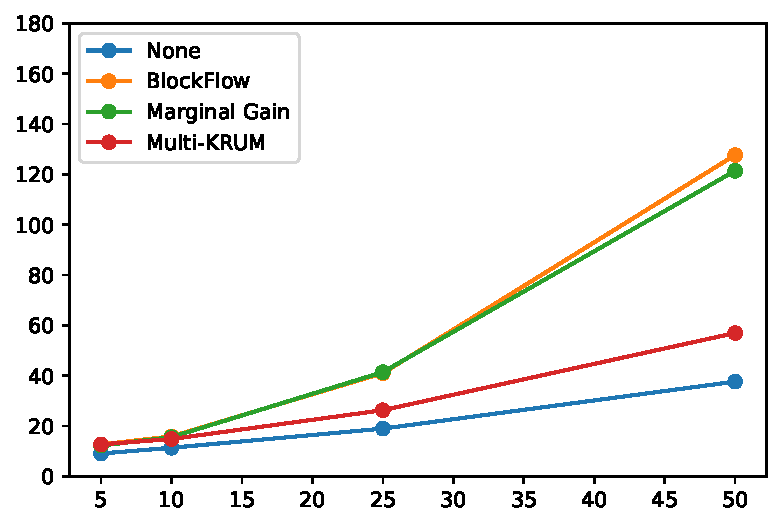
\includegraphics[width=\textwidth]{graphics/clients/e2e.pdf}
        \caption{E2E Time}
    \end{subfigure}
    \hfill
    \begin{subfigure}[b]{0.49\textwidth}
        \centering
        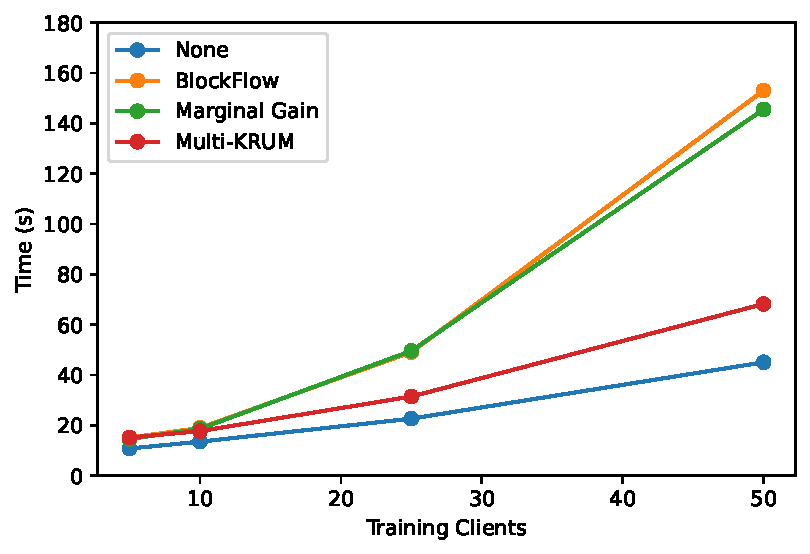
\includegraphics[width=\textwidth]{graphics/clients/round.pdf}
        \caption{Mean Round Time}
    \end{subfigure}
    \hfill
    \begin{subfigure}[b]{0.49\textwidth}
        \centering
        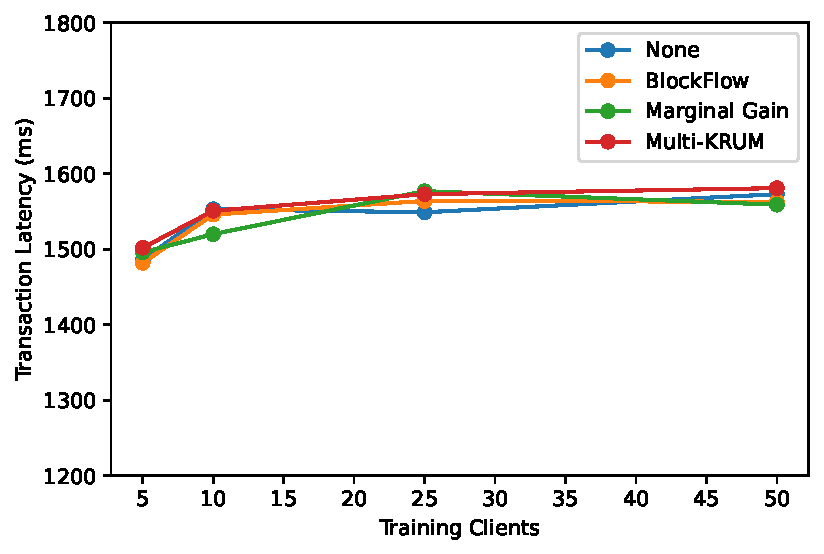
\includegraphics[width=\textwidth]{graphics/clients/tx_latency.pdf}
        \caption{Mean Transaction Latency}
    \end{subfigure}
    \hfill
    \begin{subfigure}[b]{0.49\textwidth}
        \centering
        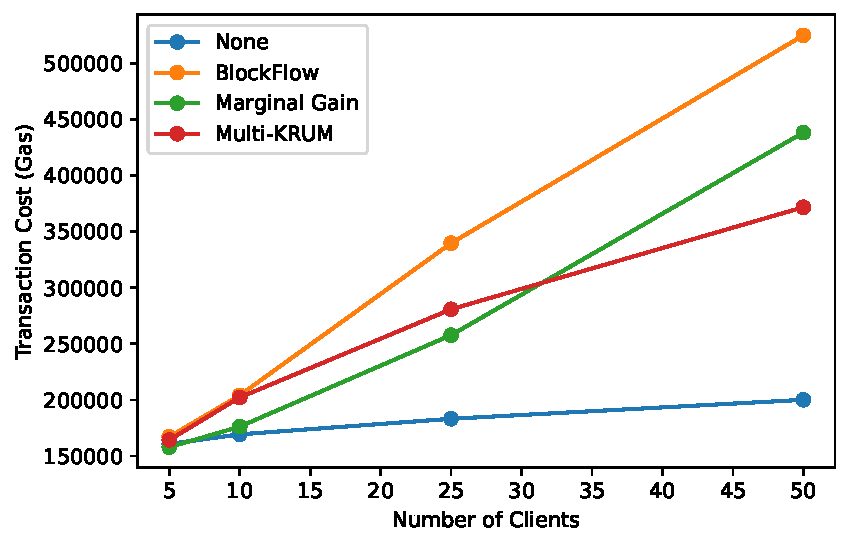
\includegraphics[width=\textwidth]{graphics/clients/tx_cost.pdf}
        \caption{Mean Transaction Cost}
    \end{subfigure}
    \caption{Time and Transaction Metrics Per Number of Clients}
    \label{fig:clients_metrics}
\end{figure}

\section{Accuracy and Convergence}

The second aspects we look at are the accuracy and how it converges along the rounds. The accuracy plots per number of clients for each scoring algorithm can be seen in \autoref{fig:accuracy_clients}.

Overall, we observe that less clients leads to a less stable convergence, that is represented by the spikes in the accuracy plots. When having a very small amount of clients, namely 5, and taking into account that the number of participants in each round is random, the model will be trained in less varied data each round. Therefore, the model can skew at some points during training, leading to a less stable convergence. In contrast, using more clients, namely 25 and 50, has an overall positive effect on both convergence stability and convergence speed. This is also likely connected to the fact that the model is trained with more varied samples from more clients in each round, leading to a better result.

Out of the three algorithms, BlockFlow seems to perform the worse. The reasons behind that phenomenon were discussed in \Cref{chapter:analysis:scoring}, where we compared the different scoring algorithms with each other.

\begin{figure}[!ht]
    \centering
    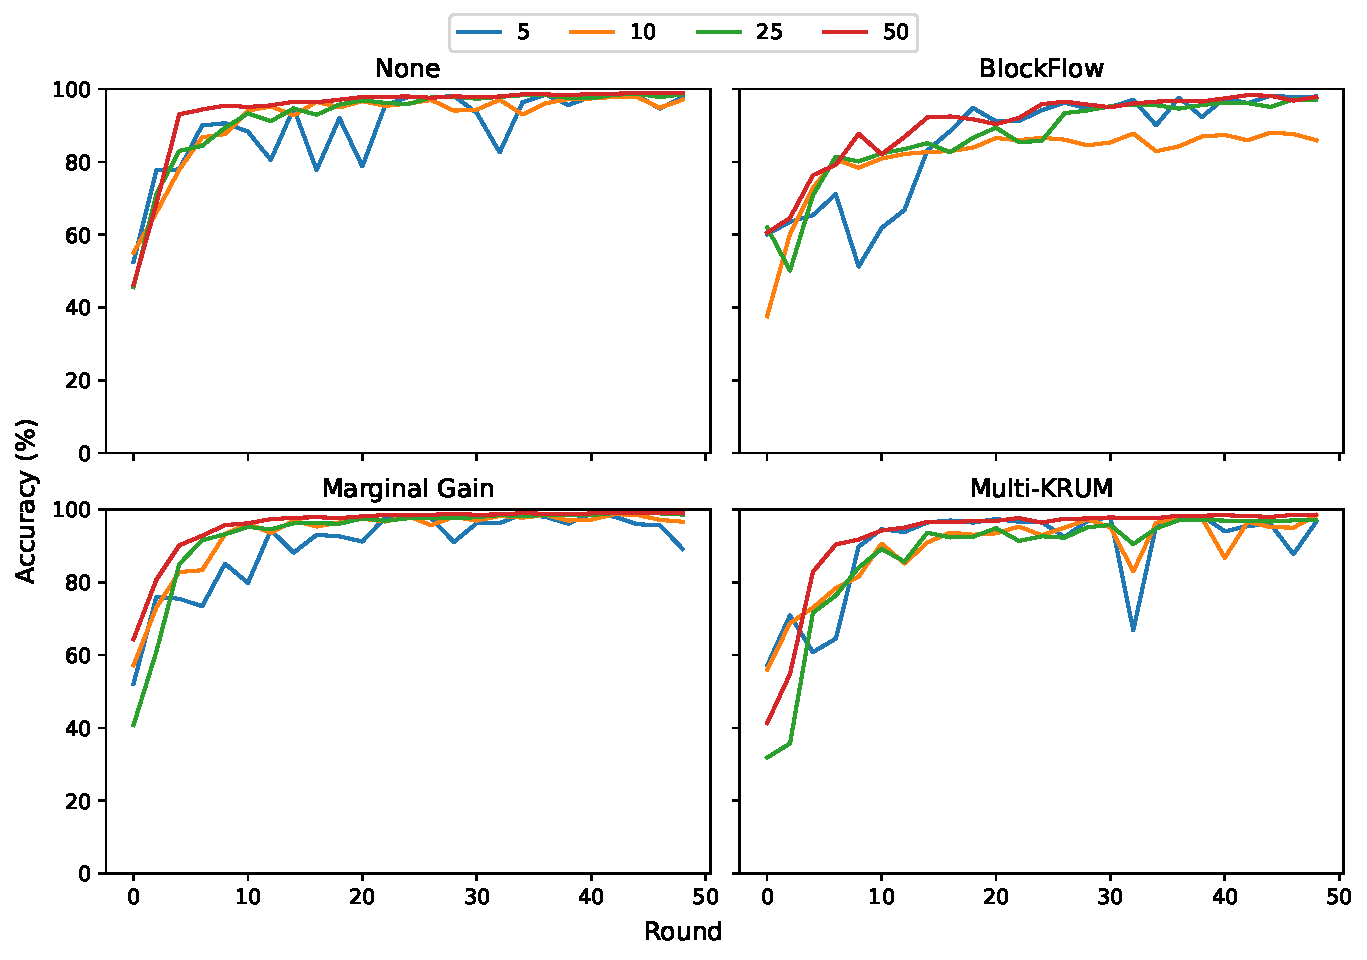
\includegraphics[width=\textwidth]{graphics/clients/accuracy.pdf}
    \caption{Accuracy Per Number of Clients}
    \label{fig:accuracy_clients}
\end{figure}

\section{Communication Costs}

The third aspect we look into are the communication costs and how they grow with the amount of clients. \autoref{fig:net_clients} depicts the network traffic required at each type of device per round per number of clients for each scoring algorithm.

In first place, we observe that, in terms of incoming traffic at the clients, there are significant changes depending on the algorithm that is used. However, the observed growth, quasi-linear, is expected. For example, in the clients, with more clients, BlockFlow and Marginal Gain have to download more weights from more clients each round to perform the scoring algorithm. In contrast, when using Multi-KRUM, which is executed by the servers, the amount of traffic per client is virtually non-changed since each client only uploads their weights once per round, which are always approximately the same size. The comparison between how much traffic is required per scoring algorithm was further discussed in \Cref{chapter:analysis:scoring}.

In second place, we observe that the incoming traffic always grows linearly in the servers when using a scoring algorithm that runs at the clients. However, when using a algorithm that runs in the server, such as Multi-KRUM, the growth is super-linear. This is explained, as we saw in \Cref{chapter:analysis:scoring} by the fact that the server will download the weights twice, one time for scoring, and another time for aggregating. As previously suggested, this can be improved by caching the weights between these two phases.

In third place, we can observe that, in terms of outgoing traffic, there are not significant differences for either the clients or the servers. In each round, the clients only upload their own weights and send a few transactions. Similarly, the servers only upload the aggregation weights and a few transactions. The small increase we observe can be explained by the additional scores that are send to the blockchain, since when there are more clients, the scorer needs to submit more scores. We can verify this by noticing that, for example, in the clients, the outgoing traffic increases more when we use scoring algorithms that are performed by the clients. Similarly, the same happens for the servers.

In fourth place, the differences observed in the blockchain process, both for incoming and outgoing traffic are negligible. With the increase on the number of clients, there are more messages going through the blockchain. However, the messages on the blockchain are very small when compared to the size of weights that need to be uploaded and downloaded by the clients and servers, respectively. 

\begin{figure}[!ht]
    \centering
    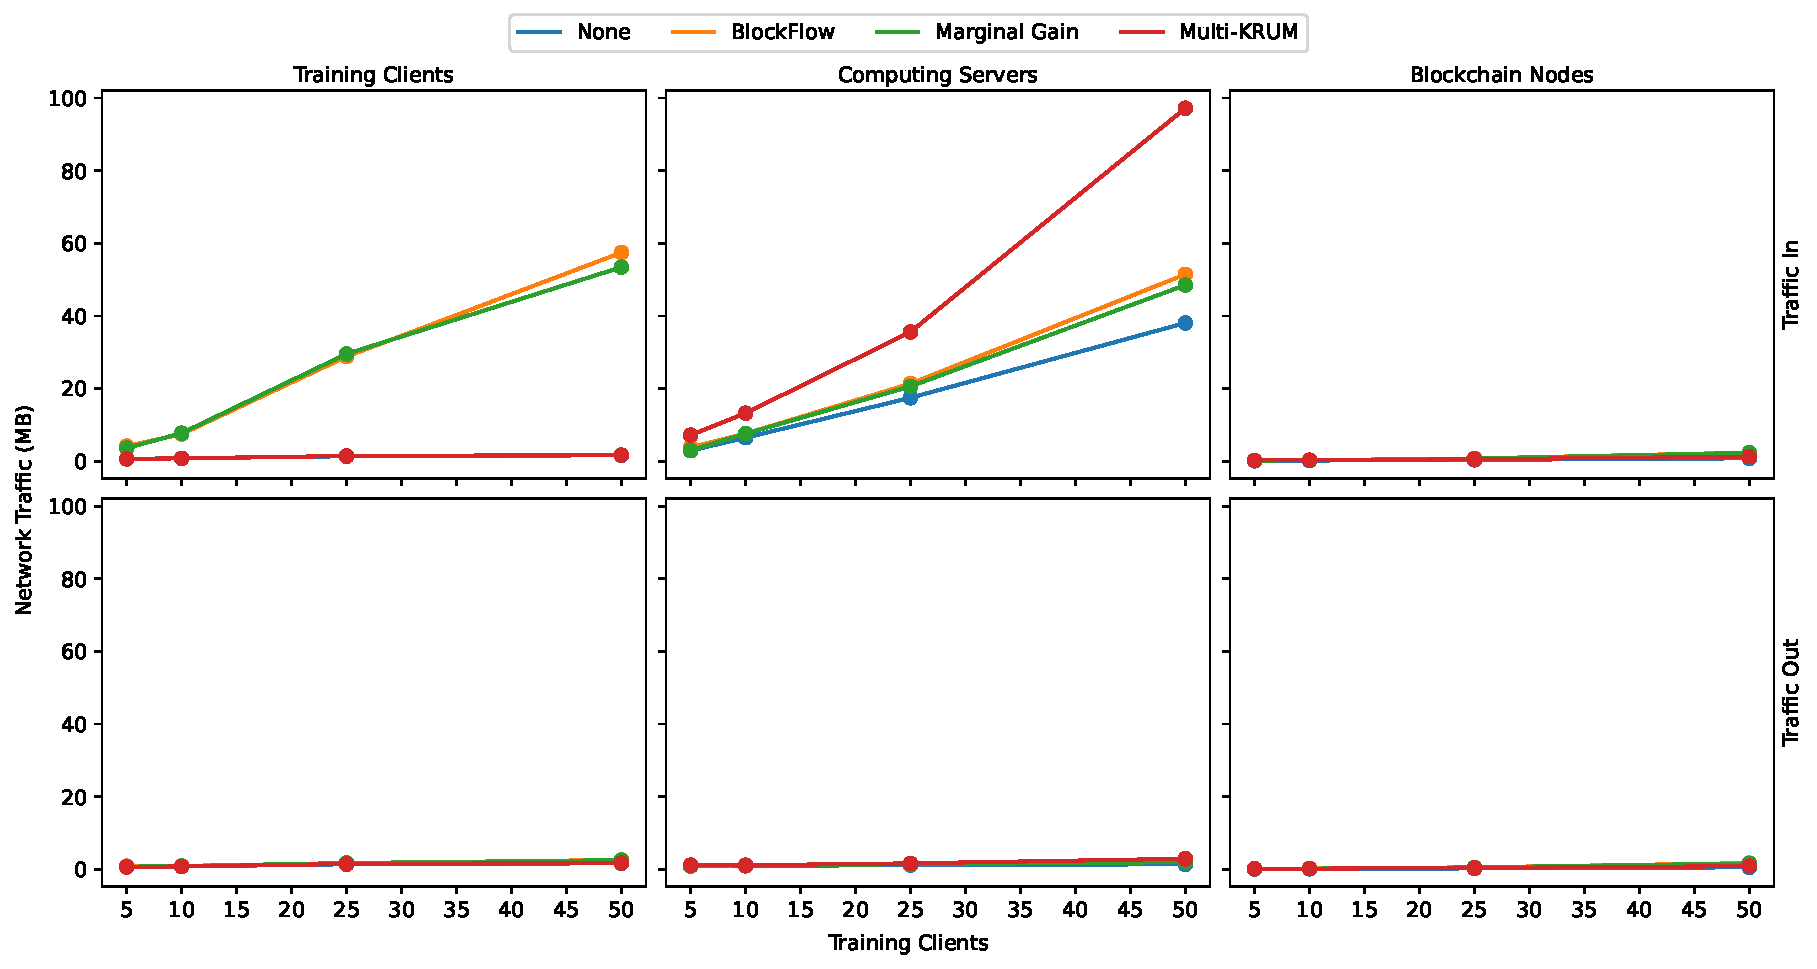
\includegraphics[width=\textwidth]{graphics/clients/traffic.pdf}
    \caption{Network Traffic Per Number of Clients}
    \label{fig:net_clients}
\end{figure}


\section{Computation Costs}

Finally, we look into the computation costs, that is, the RAM and CPU usage across the different types of devices. Since these require a large amount of plots, they are located at the end of the chapter.

Overall, the amount of clients has no major impact on either clients or servers. Even though the consumption of RAM and CPU at a certain point in time does not change wildly, there are more transactions to be processed and more scores to be calculated. Therefore, the process takes longer. By taking longer, more resources end up being consumed along the time. The growth of resource consumption is proportional to the relation between the amount of clients and the scoring algorithm. The remaining differences between scoring algorithms were discussed in \Cref{chapter:analysis:scoring}.

The only major change can be seen in the RAM and CPU usage of the blockchain process. The higher the amount of clients, the higher the RAM and CPU usage. This is expected as there are more clients connected to the blockchain, meaning more devices continuously interacting and sending transactions.

\section{Conclusions and Improvements}

In conclusion, we observed that scoring algorithms that are executed by the clients, BlockFlow and Marginal Gain, are more impacted by the increase of clients since the execution time increases super-linearly. In addition, the resource consumption at the clients increases linearly with these algorithms. In systems with low-powered devices, this may not be the best solution as the resource consumption increases.

Algorithms that are executed by the server, Multi-KRUM, do not have a major effect on the clients when the number of clients increase. However, the incoming network traffic increases super-linearly at the servers. As mentioned before, this can be improved by simply caching the weights at the servers between round phases.

Finally, the blockchain process is impacted, mainly in terms of RAM usage, by the number of clients. The more clients we have, the more resources are consumed at the blockchain process. The blockchain resource consumption is an important aspect to consider when considering using a BFS system. There is a clear trade-off between decentralization, authentication and the remaining features that are facilitated by the blockchain, with the blockchain resource consumption.

\clearpage

\begin{figure}[!h]
    \centering
    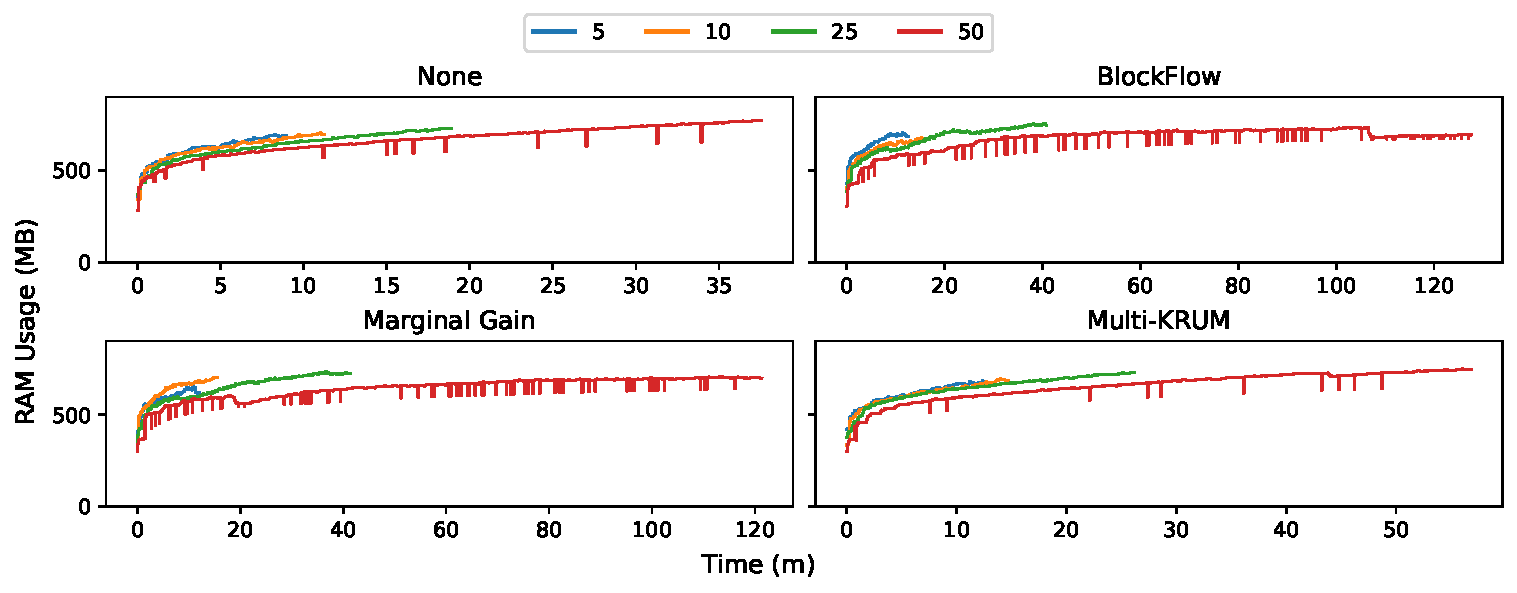
\includegraphics[width=\textwidth]{graphics/clients/ram_client.pdf}
    \caption{Client Process RAM Usage Per Number of Clients}
    \label{fig:ram_clients_clients}
\end{figure}

\vfill

\begin{figure}[!h]
    \centering
    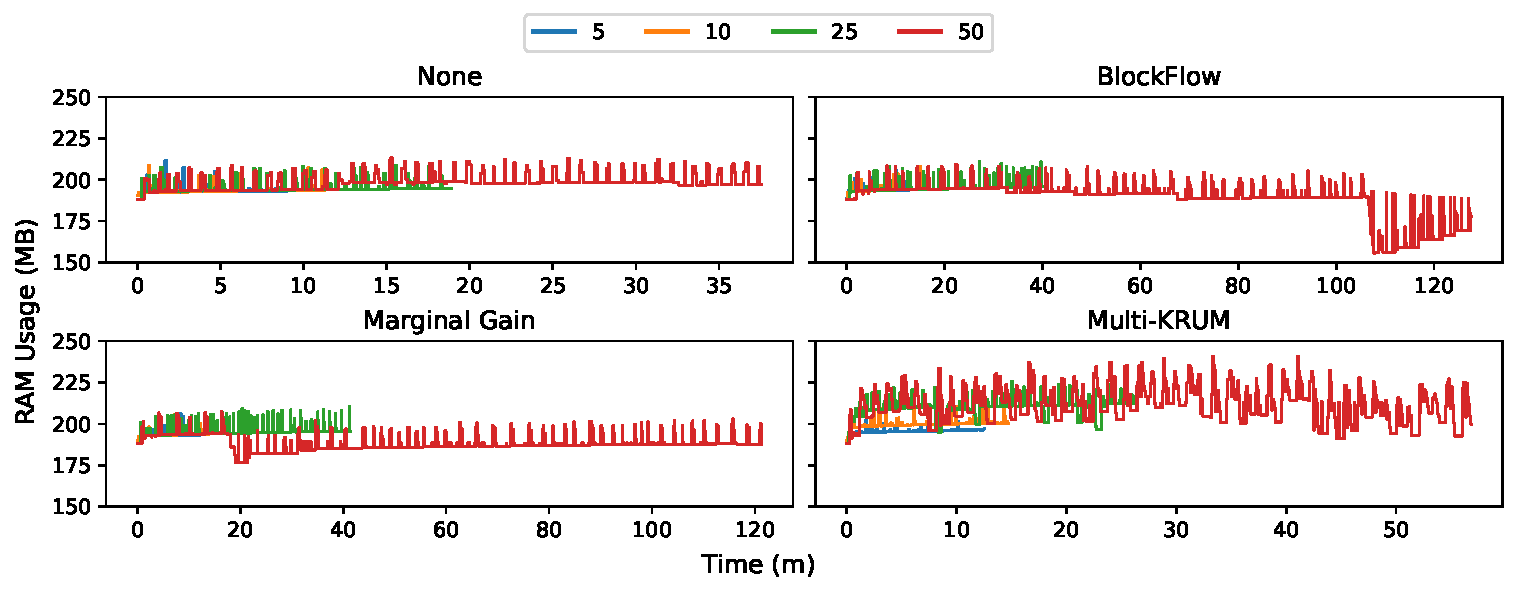
\includegraphics[width=\textwidth]{graphics/clients/ram_server.pdf}
    \caption{Server Process RAM Usage Per Number of Clients}
    \label{fig:ram_clients_servers}
\end{figure}

\vfill

\begin{figure}[!h]
    \centering
    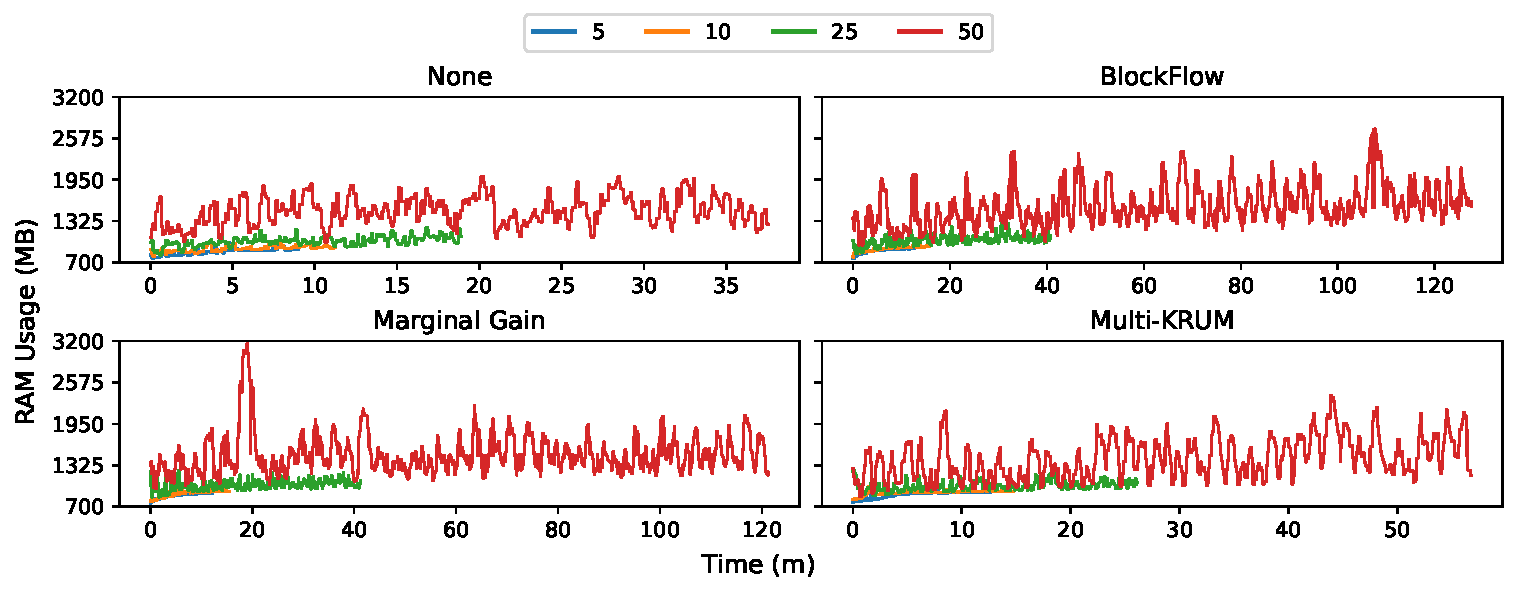
\includegraphics[width=\textwidth]{graphics/clients/ram_miner.pdf}
    \caption{Blockchain Process RAM Usage Per Number of Clients}
    \label{fig:ram_clients_miners}
\end{figure}

\clearpage

\begin{figure}[!h]
    \centering
    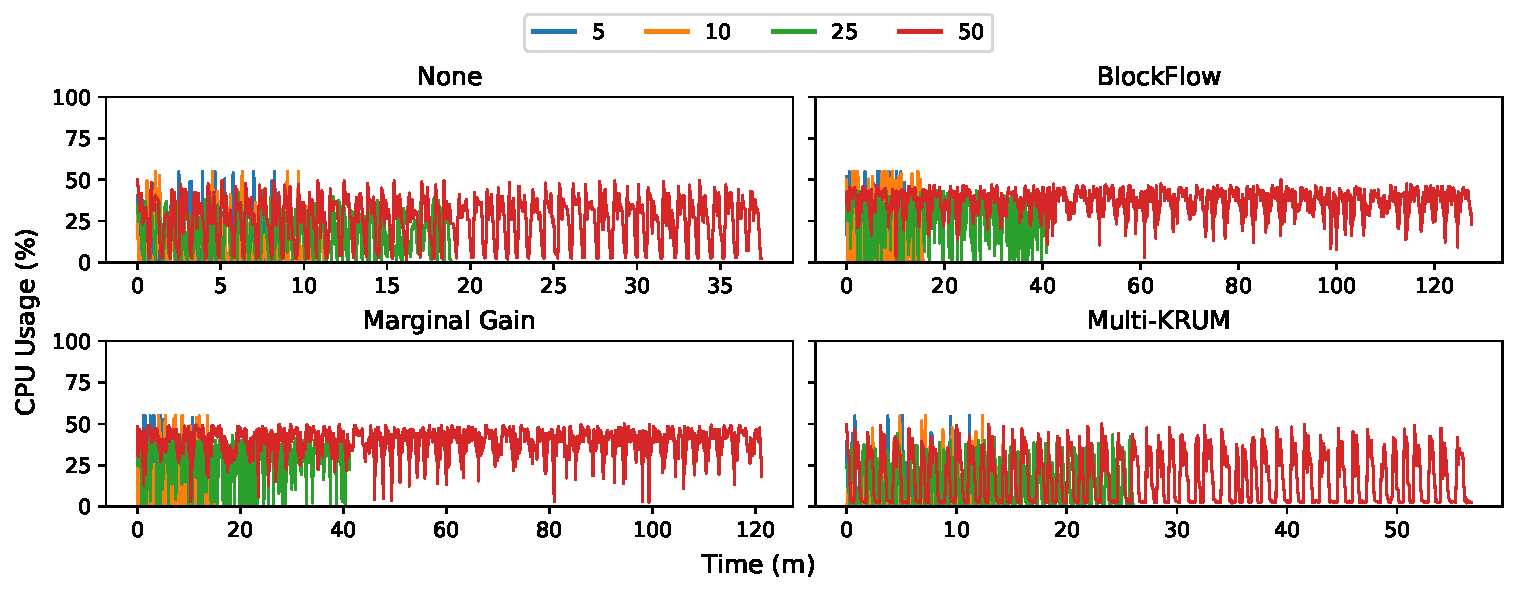
\includegraphics[width=\textwidth]{graphics/clients/cpu_client.pdf}
    \caption{Client Process CPU Usage Per Number of Clients}
    \label{fig:cpu_clients_clients}
\end{figure}

\vfill

\begin{figure}[!h]
    \centering
    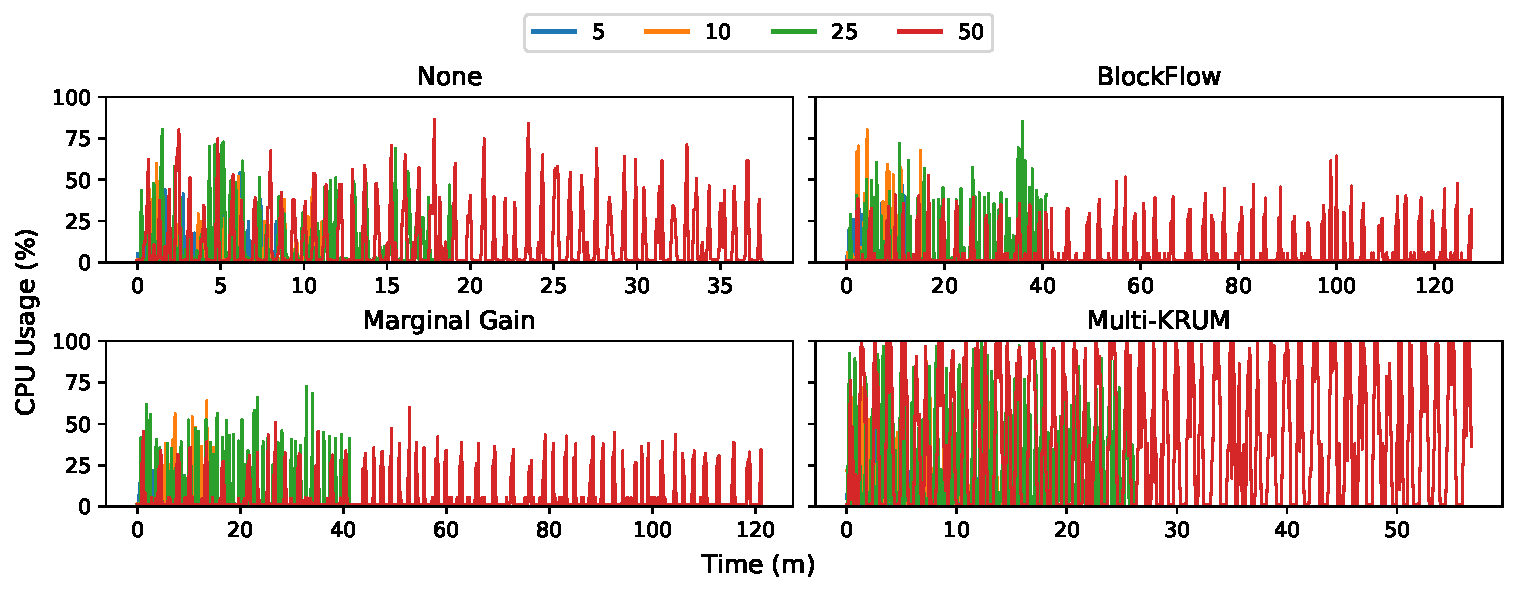
\includegraphics[width=\textwidth]{graphics/clients/cpu_server.pdf}
    \caption{Server Process CPU Usage Per Number of Clients}
    \label{fig:cpu_clients_servers}
\end{figure}

\vfill

\begin{figure}[!h]
    \centering
    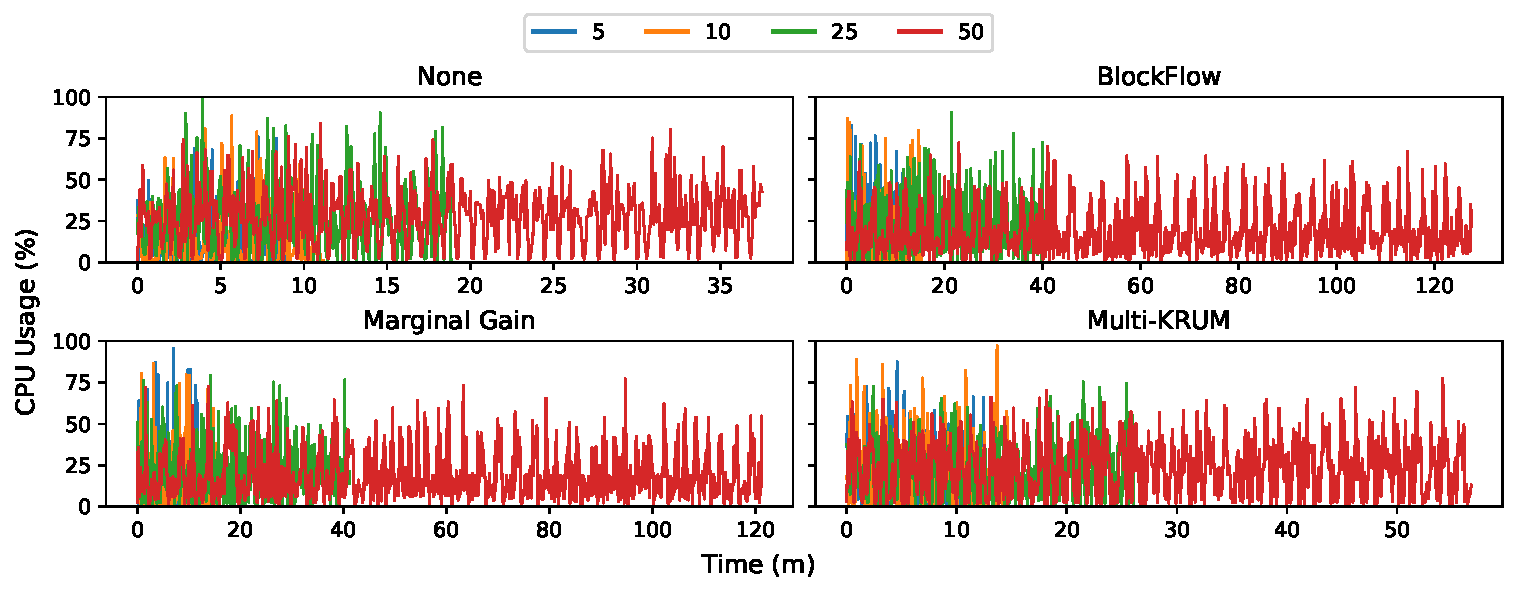
\includegraphics[width=\textwidth]{graphics/clients/cpu_miner.pdf}
    \caption{Blockchain Process CPU Usage Per Number of Clients}
    \label{fig:cpu_clients_miners}
\end{figure}

